\newpage

\section{Primera Parte: Estimación de RTT}
En esta primera parte del trabajo, el objetivo es realizar mediciones de
\emph{round-trip time} tanto teóricas como empíricas y razonar alrededor de
los resultados.

\subsection{Caracterización de los experimentos}

Elegimos tres universidades en distintas partes del mundo (Cambridge
University, Inglaterra; Stanford University, Estados Unidos; Moscow State
University, Rusia) y, tomando la dirección IP del dominio principal de cada
una, realizamos las siguientes mediciones:
\begin{enumerate}
    \item Cálculo del RTT teórico. Para esto, primero definimos la ubicación
        geográfica de la dirección haciendo uso de un servicio de
        geolocalización. Con ella, calculamos la distancia lineal desde ese
        punto hasta el que sería el origen de nuestras mediciones. Tomando un
        tiempo de propagación de la señal de $2 \times 10^5$ km/s, calculamos
        el tiempo que tardaría la ida de un paquete hasta el servidor destino
        y la llegada de una respuesta.
    \item Medición de RTT mediante una herramienta propia. Utilizando una
        herramienta de \emph{traceroute} desarrollada por nosotros usando la
        biblioteca Scapy, calculamos el RTT empírico a la dirección destino.
    \item Medición de RTT mediante una herramienta del sistema operativo.
        Idéntico al caso anterior pero esta vez usando el \emph{traceroute}
        disponible en una distribución de GNU/Linux.
    \item Medición de RTT teórico teniendo en cuenta el camino recorrido por
        los paquetes. Similar al cálculo teórico anterior, esta vez teniendo
        en cuenta las ubicaciones geográficas de cada uno de los routers
        intermedios.
\end{enumerate}

Previamente a las mediciones, se esperaba que el RTT teórico lineal fuera, en
general, muy menor a los obtenidos empíricamente, puesto que este, además de
dejar de lado retardos ocasionados por los routers en distintas horas del día,
asumía la existencia de un medio de comunicación (fibra óptica) cubriendo la
menor distancia entre el origen y el destino de la medición. Dado que el RTT
teórico del camino no asume esto último, se esperaba que este se ajustara más
a los valores empíricos. Por otro lado, se esperaba ver que los valores de RTT
empíricos arrojados por ambas herramientas de \emph{traceroute} fueran
cercanos, ya que las mediciones se realizarían en condiciones similares y los
métodos para realizar los cálculos serían similares.

Asimismo, como realizaríamos mediciones para distintos momentos del día, se
esperaba ver diferencias en los RTT según el horario, aunque no se suponía
ningún patrón en particular.

\subsection{Resultados de los experimentos}

Los gráficos \ref{fig:cambridge:count}, \ref{fig:stanford:count} y
\ref{fig:msu:count} muestran las mediciones para la Cambridge University
(Inglaterra), Stanford University (Estados Unidos) y la Moscow State
University (Rusia) respectivamente. En ellos pueden verse los valores para
distintos horarios del día.

\begin{figure}[h!]
    \centering
    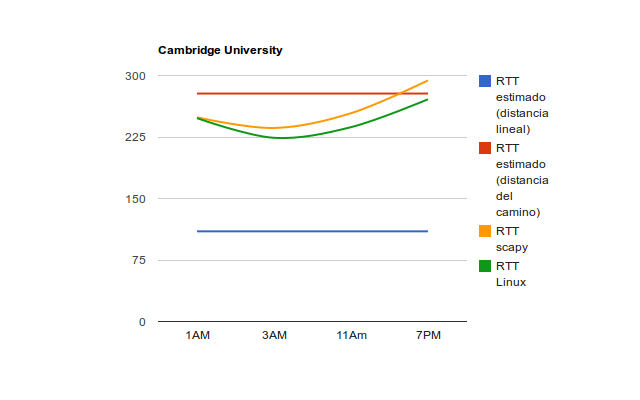
\includegraphics[width=400pt]{cambridge.png}
    \caption{Cambridge University}
    \label{fig:cambridge:count}
\end{figure}

\begin{figure}[h!]
    \centering
    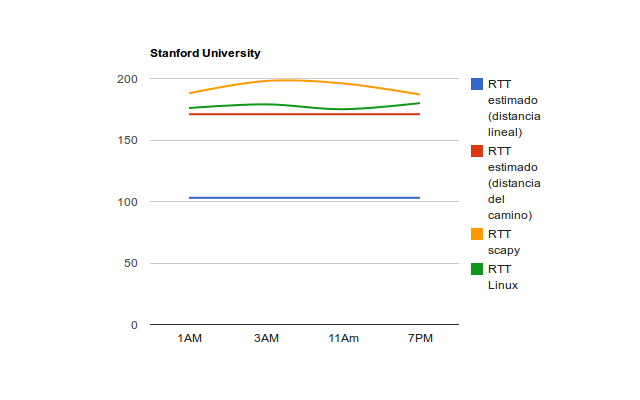
\includegraphics[width=400pt]{stanford.png}
    \caption{Stanford University}
    \label{fig:stanford:count}
\end{figure}

\begin{figure}[h!]
    \centering
    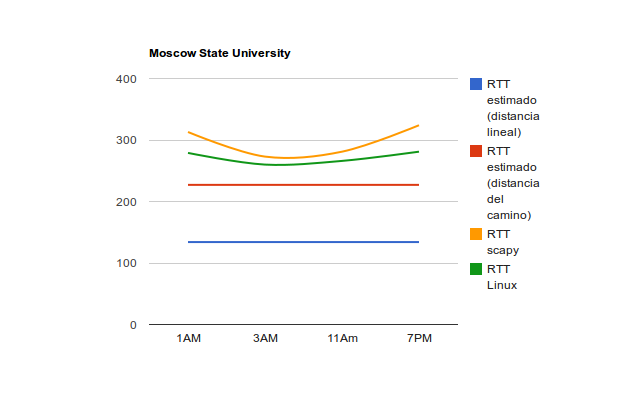
\includegraphics[width=400pt]{msu.png}
    \caption{Moscow State University}
    \label{fig:msu:count}
\end{figure}

\subsection{Análisis de los resultados}

\indent Nos pareció interesante saber cuantos km de mas tuvimos que recorrer dado que, por razones obvias, no tenemos un enlace punto a punto desde nuestras casas hacia el destino. Es por eso que están graficados ambos RTTs teóricos, creimos que tomando la distancia recorrida hasta llegar a destino iba a dar un RTT más ajustado a la realidad y así fue.\\

\indent Lo primero que se observa es como a la madrugada el RTT es menor en las dos rutas hacia Europa debido a que en ese horario el tráfico es menor tanto en el origen como en el destino, esto no sucede en la ruta hacia Estados Unidos ya que al ser en la costa oeste 4hs menos que en Buenos Aires a esa hora todavía se registra un tráfico mayor.\\

\indent En el primer gráfico llama la atención que el RTT teórico sea superior en algunos casos al RTT observado, creemos que esto se debe a un posible error en la herramienta de geolocalización ya que hay un desvío de unos 1000km en uno de los últimos hops. También puede estar sucediendo que ese hop, que tiene una IP de Escocia, en realidad sea un servidor que está en Inglaterra pero por alguna razón tiene una IP de ese país. Lo mismo sucede con uno de los primeros hops, que tiene una IP de Estados Unidos pero el RTT medido es de 28ms.\\

\indent Por último vimos que los resultados de las dos herramientas son bastante similares, probablemente el hecho de que la implementación de Traceroute del sistema operativo haga 3 intentos por hop sea la razón por la cual su curva sea más suave.\\

